\section{参数敏感性}
\label{sec:opt-lp-sensitivity}

模型中的数据往往只是估计：明天的原料可能多到一些，产品价格可能变动。重新求解当然可以，但我们更想知道，已经求得的最优基在多大范围内仍然有效，最优值又以什么速率变化。本节固定约束矩阵$\bm A$，分别改变右端$\bm b$和目标系数$\bm c$。之所以把$\bm A$固定，是因为改变资源数量与改变单位产品的资源消耗是两种不同的扰动：前者只移动约束边界，后者改变边界的方向，会同时影响可行性和比较，需要另作分析。

两种改变的检查方法都来自同一个观察：基$B$保持最优，当且仅当它同时满足两组条件，即基本解可行（$\bm A_B^{-1}\bm b\ge\bm 0$）与约化费用非负（$\bm c_N-\bm A_N^\top\bm A_B^{-\top}\bm c_B\ge\bm 0$）。前一组只涉及$\bm b$，后一组只涉及$\bm c$。所以改变$\bm b$只需重新检查可行性，改变$\bm c$只需重新检查约化费用。

\subsection{约束右端的变化}
\label{sec:opt-lp-rhs}

\paragraph{原基保持最优的范围}
把右端改为$\bm b+\Delta\bm b$，保留原最优基$B$。约化费用只依赖$\bm A$与$\bm c$，没有变化，对偶解$\bm y=\bm A_B^{-\top}\bm c_B$也仍然对偶可行。变化的只是基本解：
\[
  \bm x_B(\Delta\bm b)=\bm A_B^{-1}(\bm b+\Delta\bm b).
\]
只要它非负，$B$就仍是可行基，而约化费用非负，于是$B$仍然最优。这组线性不等式就是$\Delta\bm b$的允许范围。

在资源模型中，原最优基$B=\{1,2\}$，$\bm A_B^{-1}=\tfrac13\bigl(\begin{smallmatrix}2&-1\\-1&2\end{smallmatrix}\bigr)$。只改变第一种原料，$b_1=4+\delta$，得
\[
  x_1=\frac{2(4+\delta)-4}{3}=\frac{4+2\delta}{3},\qquad
  x_2=\frac{-(4+\delta)+8}{3}=\frac{4-\delta}{3},
\]
二者非负当且仅当$-2\le\delta\le4$，即$b_1\in[2,8]$。在这个范围内，最优产量沿直线$x_1+2x_2=4$移动：第一种原料越多，越多地生产更耗它的第一种产品。图~\ref{fig:opt-lp-rhs-sensitivity}(a)画出了这一移动，$b_1=2$时最优点到达$(0,2)$，$b_1=8$时到达$(4,0)$。

\paragraph{影子价格}
在允许范围内，最优值为
\[
  \bm c_B^\top\bm A_B^{-1}(\bm b+\Delta\bm b)=\bm y^\top\bm b+\bm y^\top\Delta\bm b,
\]
增量是$\bm y^\top\Delta\bm b$。对偶变量于是有了直接的含义：$y_i$是第$i$个右端每增加一个单位时最优值的变化率。在资源模型的最大化写法中，最优获利为$\tfrac{20}3+\tfrac43\delta$：第一种原料每多一个单位，获利多$4/3$，这正是对偶解给它的价格$u_1=4/3$；同理第二种原料每单位值$u_2=1/3$，其允许范围也是$b_2\in[2,8]$。因此对偶最优解又称\term{影子价格}（shadow price）：它告诉作坊，在当前范围内，为多买一单位原料最多值得付多少钱。第二种原料的影子价格只有$1/3$，若市价高于此，就不值得为它扩产。

\paragraph{超出范围之后}
影子价格只在允许范围内有效。图~\ref{fig:opt-lp-rhs-sensitivity}(b)画出了最优获利$v(b_1)$在整个范围内的变化：
\[
  v(b_1)=\begin{cases}
    2b_1, & 0\le b_1\le2,\\[2pt]
    \tfrac{4b_1+4}{3}, & 2\le b_1\le8,\\[2pt]
    12, & b_1\ge8.
  \end{cases}
\]
$b_1<2$时原基给出$x_1<0$，需要换基，最优点变为$(0,b_1)$，此时只生产第二种产品，第一种原料是唯一的瓶颈，它的价格升到$2$；$b_1>8$时原基给出$x_2<0$，最优点停在$(4,0)$，第一种原料已经过剩，价格降为$0$。$b_1<0$时问题不可行。函数在$b_1=2$与$b_1=8$处有折点，各段斜率正是相应最优基的影子价格。在折点上，最优对偶解不唯一：例如$b_1=2$时，价格$(2,0)$与$(4/3,1/3)$给出的总价都是$4$，它们分别是左、右两侧的斜率。这时只说“影子价格是多少”已经不准确，左右的变化率并不相同。

\begin{figure*}[!htbp]
  \centering
  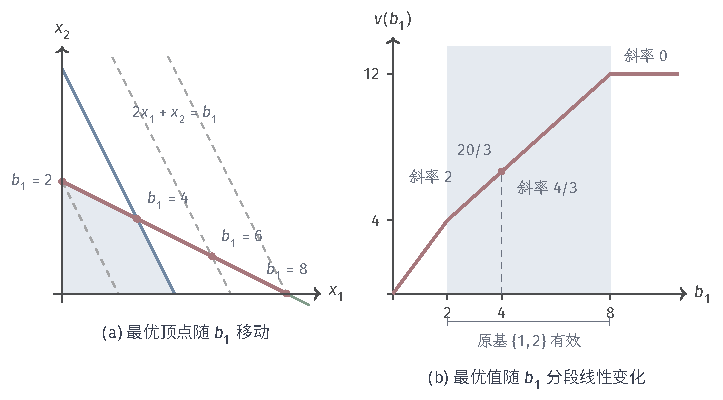
\includegraphics[width=122.357mm]{figures/03-optimization-evolution-and-signals/01-optimization/tikz/c2-rhs-sensitivity/figure.pdf}
  \caption{改变第一种原料的数量$b_1$（第二种固定为$4$）。(a) 蓝线是$b_1=4$时的边界$2x_1+x_2=4$，灰色虚线是$b_1=2,6,8$时的边界；红点是相应的最优顶点$((2b_1-4)/3,(8-b_1)/3)$，它们沿红线$x_1+2x_2=4$从$(0,2)$移到$(4,0)$。(b) 最优获利$v(b_1)$分三段线性变化，斜率依次为$2$、$4/3$、$0$；浅蓝区域$b_1\in[2,8]$内原基保持最优，斜率$4/3$就是第一种原料的影子价格，红点为$b_1=4$时的值$20/3$。}
  \label{fig:opt-lp-rhs-sensitivity}
\end{figure*}

这条折线是凹的，这不是巧合。若右端为$\bm b$与$\bm b'$时的最优解分别是$\bm x$与$\bm x'$，则对$\lambda\in[0,1]$，$\lambda\bm x+(1-\lambda)\bm x'$满足右端为$\lambda\bm b+(1-\lambda)\bm b'$的约束，所以最大化问题的最优值满足$v(\lambda\bm b+(1-\lambda)\bm b')\ge\lambda v(\bm b)+(1-\lambda)v(\bm b')$。凹性说明影子价格随资源增多而不增：资源越充裕，再多一单位的价值越低。对任意大的变化，影子价格仍然给出一个可靠的单侧界：设$\bm u$是右端为$\bm b$时的最优价格，它的可行性与右端无关，由弱对偶，对任何使问题可行的$\bm b'$都有$v(\bm b')\le\bm u^\top\bm b'=v(\bm b)+\bm u^\top(\bm b'-\bm b)$。所以“当前价格乘以变化量”在最大化问题中只是增量的上界，越出允许范围后可能严重高估，不能当作精确的预测。

\subsection{目标系数的变化}
\label{sec:opt-lp-cost}

\paragraph{原基保持最优的范围}
现在固定$\bm A$与$\bm b$，把目标系数改为$\bm c+\Delta\bm c$。原基本解$\bm A_B^{-1}\bm b$与$\bm c$无关，仍然可行；需要重新检查的是约化费用
\[
  \bar{\bm c}_N(\Delta\bm c)=(\bm c_N+\Delta\bm c_N)-\bm A_N^\top\bm A_B^{-\top}(\bm c_B+\Delta\bm c_B)\ge\bm 0.
\]
这一次保持不变的是可行点，重新变化的是候选之间的比较。

在资源模型中把第一种产品的获利改为$c_1$，最大化$c_1x_1+2x_2$。标准型中$\bm c_B=(-c_1,-2)^\top$，解$\bm A_B^\top\bm y=\bm c_B$得
\[
  y_1=\frac{2-2c_1}{3},\qquad y_2=\frac{c_1-4}{3},
\]
于是两个松弛变量的约化费用为$\bar c_3=-y_1=\tfrac{2c_1-2}3$、$\bar c_4=-y_2=\tfrac{4-c_1}3$。二者非负当且仅当$1\le c_1\le4$。在这个范围内顶点$(4/3,4/3)$保持最优，$c_1=3$时回到原来的数值$\bar c_3=4/3$、$\bar c_4=1/3$。

\paragraph{最优性锥}
这个范围有一个直观的几何解释。在顶点$(4/3,4/3)$处活跃的两条约束的外法向量是$(2,1)$与$(1,2)$。上面算出的$-\bm y$满足
\[
  (c_1,2)=\frac{2c_1-2}{3}(2,1)+\frac{4-c_1}{3}(1,2),
\]
即目标方向被写成两个法向量的组合，组合系数正是两种原料的价格。系数都非负，等价于目标方向落在两个法向量张成的锥中。图~\ref{fig:opt-lp-cost-sensitivity}(a)画出了这个锥：$c_1=3$的方向$(3,2)$在锥内，顶点最优；$c_1=6$的方向$(6,2)$转出了锥，沿边走向$(2,0)$会更好。$c_1=4$时方向$(4,2)$落在锥的边界上，与边$2x_1+x_2=4$垂直，$\bar c_4=0$，整条边都最优，这正是图~\ref{fig:opt-lp-optimal-face}(b)的情形（目标乘以正数不改变最优解）。$c_1=1$时方向$(1,2)$落在另一条边界上，最优面是通往$(0,2)$的边。

\paragraph{最优值的变化}
在原基保持最优的范围内，最优解不变，最优值随系数线性变化，变化率就是相应变量的取值：最大化写法中$v(c_1)=\tfrac43c_1+\tfrac83$，每件第一种产品多获利一单位，总获利多$x_1^\star=4/3$。当某个约化费用降到零时，出现多个最优解，再越过这一点就要换基。图~\ref{fig:opt-lp-cost-sensitivity}(b)画出了$v(c_1)$在整个范围内的变化：$c_1\le1$时最优点是$(0,2)$，$v=4$；$1\le c_1\le4$时是$(4/3,4/3)$；$c_1\ge4$时是$(2,0)$，$v=2c_1$。这里的折线是凸的，因为$v(c_1)$是有限个基本可行解上线性函数$c_1x_1+2x_2$的最大值。

\begin{figure*}[!htbp]
  \centering
  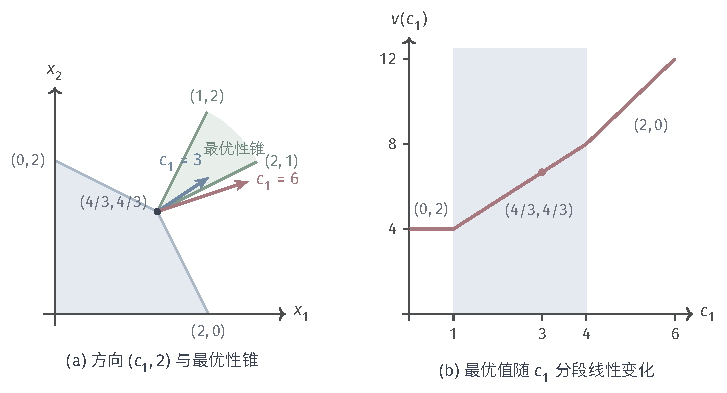
\includegraphics[width=123.126mm]{figures/03-optimization-evolution-and-signals/01-optimization/tikz/c2-cost-sensitivity/figure.pdf}
  \caption{改变第一种产品的获利$c_1$（第二种固定为$2$）。(a) 在顶点$(4/3,4/3)$处，两条活跃约束的外法向$(2,1)$与$(1,2)$张成绿色的最优性锥；目标方向$(c_1,2)$落在锥内时这个顶点最优。蓝色箭头$c_1=3$在锥内，红色箭头$c_1=6$在锥外；$c_1=4$与$c_1=1$恰好对应锥的两条边。(b) 最优获利$v(c_1)$分三段线性变化，各段旁标出最优顶点；浅蓝区域$c_1\in[1,4]$内原基保持最优，斜率为$x_1^\star=4/3$。}
  \label{fig:opt-lp-cost-sensitivity}
\end{figure*}

\paragraph{两种变化的对照}
右端变化与目标系数变化限制原基的方式不同。改变$\bm b$时约化费用不动，原基失效的原因是基本解出现负分量，即原来的顶点已不可行；最优值对$\bm b$的变化率是对偶解$\bm y$，值函数（最大化写法中）是凹的。改变$\bm c$时基本解不动，原基失效的原因是某个约化费用变负，即沿某条边可以改进；最优值对$\bm c$的变化率是原始解$\bm x$，值函数是凸的。两种条件不能互换：资源数量在允许范围内变动时，最优基不变，最优产量却按$\bm A_B^{-1}(\bm b+\Delta\bm b)$移动；产品价格在允许范围内变动时，最优基和最优产量都完全不动，变的只是获利。
